\chapter{METHODOLOGY AND IMPLEMENTATION WORKFLOW}
The proposed system combines deep learning, computer vision, IoT sensing, and Explainable AI techniques for automated food spoilage detection and monitoring. The methodology involves dataset collection, preprocessing, augmentation, model training, IoT integration, prediction fusion, Explainable AI visualization, and web-based deployment. The complete workflow is designed to perform multi-label spoilage classification of fruits and vegetables while incorporating environmental sensing for improved prediction reliability. The chapter discusses the overall system workflow, implementation methodology, and technologies used in the proposed system.

\section[Overall Methodology]{\textbf{Overall Methodology}}
The methodology is structured as an end-to-end pipeline that synchronizes visual data with environmental sensor telemetry. The process begins with automated data ingestion from a local camera module and the IoT sensor array. Images are streamed as NumPy arrays, while sensor data (temperature, humidity, and VOC levels) are transmitted via Serial communication from the ESP32 to the host machine. This dual-stream approach ensures that the system has access to both the 'symptoms' of spoilage (visual indicators) and the 'causes' (environmental conditions).

The integration of these disparate data sources is managed by a centralized Python-based processing engine. The engine coordinates the execution of the deep learning inference and the sensor risk calculation in parallel, minimizing latency. This architecture supports real-time monitoring, where the prediction is updated dynamically as the environment changes, making it suitable for active storage tracking in smart kitchens and warehouses.

\begin{figure}[H]
	\centering
	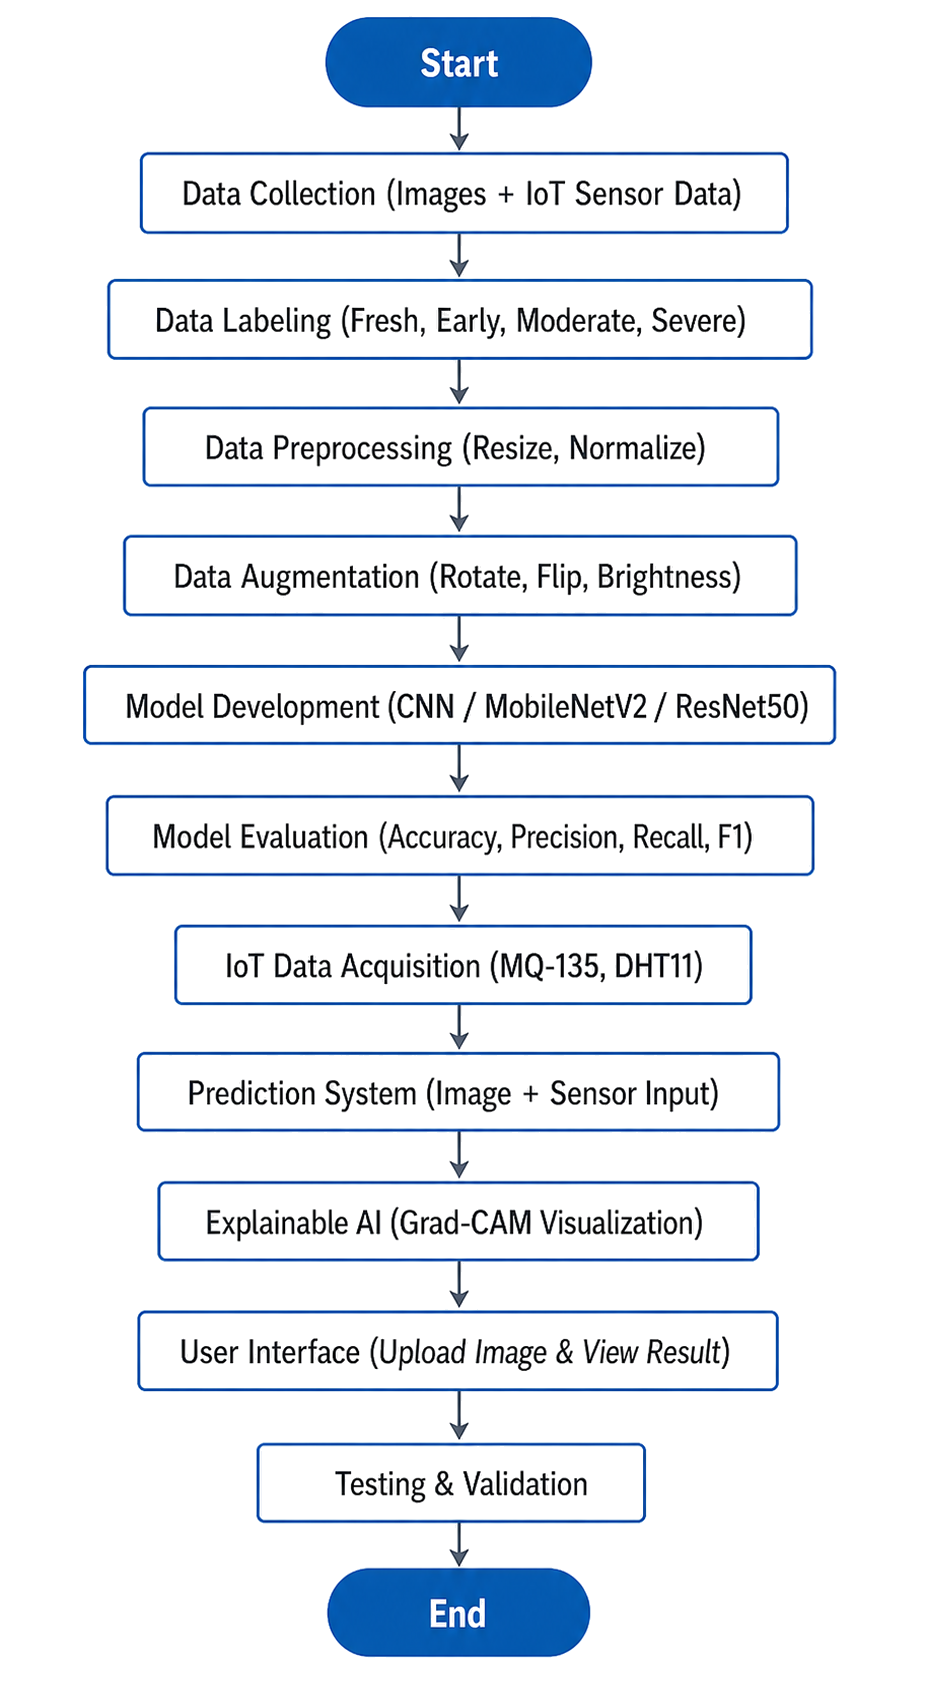
\includegraphics[width=0.45\textwidth]{Figures/methodology_image_transparent}
	\caption{Flowchart of the proposed AI-based multi-label food spoilage detection and IoT fusion methodology.}
	\label{fig:methodology_workflow_diagram}
\end{figure}

\begin{table}[H]
	\centering
	\caption{Methodology Workflow of the Proposed System}
	\label{tab:methodology_workflow}
	\begin{tabular}{|l|l|}
		\hline
		\textbf{Stage} & \textbf{Description} \\ \hline
		Data Collection & Collection of fruit and vegetable images from public datasets \\ \hline
		Data Labeling & Classification into Fresh, Early, Moderate, and Severe spoilage stages \\ \hline
		Preprocessing & Image resizing, normalization, and cleaning \\ \hline
		Data Augmentation & Rotation, flipping, zooming, and brightness adjustment \\ \hline
		Model Training & Training CNN and transfer learning models \\ \hline
		IoT Integration & Collection of environmental data using sensors \\ \hline
		Sensor Fusion & Combination of image prediction and sensor risk score \\ \hline
		Explainable AI & Grad-CAM visualization for prediction interpretation \\ \hline
		Deployment & Streamlit-based web application development \\ \hline
	\end{tabular}
\end{table}

\section[Deep Learning Workflow]{\textbf{Deep Learning Workflow}}
The deep learning training pipeline is optimized for high accuracy on multi-label classification. The models are implemented using the \textit{Keras} API with the following training configurations:
\begin{itemize}
    \item \textbf{Loss Function}: Categorical Cross-Entropy, as it is a multi-class classification problem.
    \item \textbf{Optimizer}: \textit{Adam} optimizer, starting with a learning rate of $0.001$.
    \item \textbf{Fine-tuning}: After initial training of the top layers, the backbone layers (e.g., in MobileNetV2) are unfrozen and trained with a reduced learning rate of $10^{-5}$ to refine the lower-level features without destroying the pretrained weights.
    \item \textbf{Regularization}: Dropout layers (rate: 0.5) and L2 weight regularization are added to prevent the model from memorizing the training samples.
\end{itemize}
The training is performed with a batch size of 32 for 50 epochs, utilizing an \textit{EarlyStopping} callback to halt training once the validation loss plateaus for more than 5 consecutive epochs.

\section[IoT Data Acquisition and Sensor Integration]{\textbf{IoT Data Acquisition and Sensor Integration}}
The IoT subsystem is designed for low-power, high-accuracy sensing. The microcontroller (ESP8266 or ESP32) samples data from the sensor array at a frequency of 1 Hz (2-second measurement intervals). To eliminate high-frequency electronic noise and jitters in the MQ-135 and DHT22 readings, a simple moving average filter with a window size of 5 is implemented on the firmware side.

The risk estimation logic is defined by a rule-based engine:
\begin{itemize}
    \item \textbf{Thresholds}: Spoilage risk is flagged if Temperature exceeds $30^{\circ}C$, Humidity exceeds 80\%, or VOC levels (from MQ-135) cross 200-400 ppm.
    \item \textbf{Risk Scoring}: These individual factors are combined into a normalized $[0, 1]$ risk score. This score represents the 'Environmental Spoilage Probability'.
\end{itemize}

The firmware integrates with the Blynk IoT cloud platform for real-time sensor monitoring and alert triggering. Virtual pins on Blynk display live gas concentration, temperature, and humidity readings. When spoilage conditions are detected, the system triggers cloud events that send push notifications and email alerts to the user. A local 16x2 I2C LCD display and tri-color LED indicator provide immediate visual feedback at the device level. The complete ESP8266/Arduino firmware implementation is provided in Appendix Section A.8.

The sensor data is also formatted into a JSON string and sent to the Streamlit application via a virtual COM port or MQTT protocol, where it is used to adjust the final prediction confidence in the fusion module.

\begin{table}[H]
	\centering
	\caption{IoT Sensors Used in the Project}
	\label{tab:iot_sensors}
	\begin{tabular}{|l|l|l|}
		\hline
		\textbf{Sensor} & \textbf{Parameter Monitored} & \textbf{Purpose} \\ \hline
		MQ-135 & Gas concentration & Detection of spoilage-related gases \\ \hline
		DHT11/DHT22 & Temperature and Humidity & Monitoring environmental conditions \\ \hline
		ESP32 / Arduino Uno & Sensor interfacing & Data acquisition and transmission \\ \hline
	\end{tabular}
\end{table}

\section[Explainable AI and Prediction System]{\textbf{Explainable AI and Prediction System}}
The final prediction system employs a \textit{Late Fusion} strategy. The image classification model outputs a probability distribution $P_{DL}$ across the four classes, and the IoT risk score $R_{env}$ provides a weight adjustment factor.
\begin{equation}
    P_{final} = Softmax(P_{DL} + \lambda \cdot R_{env})
\end{equation}
where $\lambda$ is a hyperparameter determined through validation to balance the influence of sensor data.

To provide user-centric explainability, \textbf{Grad-CAM} generates a saliency map of the input image. This map is calculated by taking the gradient of the winning class with respect to the feature maps of the last convolutional layer. The resulting heatmap is upsampled to $224 \times 224$ and superimposed on the original image using a 40\% transparency alpha-blend. This allows the user to see exactly where the mold or discoloration was detected, transforming the system from a 'black box' into a transparent diagnostic tool. Finally, the Streamlit UI displays the real-time sensor charts, the prediction gauge, and the Grad-CAM output in a unified dashboard.

\section[Detailed Hardware Configuration]{\textbf{Detailed Hardware Configuration}}
This section provides comprehensive hardware implementation details including component specifications, wiring diagrams, sensor calibration thresholds, and cloud platform configuration for the IoT subsystem.

\subsection{Hardware Components and Specifications}
The IoT monitoring subsystem employs the following components:
\begin{itemize}
    \item \textbf{Microcontroller}: NodeMCU ESP8266 with built-in Wi-Fi capability for cloud connectivity and real-time data transmission
    \item \textbf{Gas Sensor}: MQ-3/MQ-135 for detecting alcohol vapors, ammonia, and volatile organic compounds (VOCs) emitted during food decomposition with analog output range 0-1023
    \item \textbf{Environmental Sensor}: DHT11 for temperature and humidity monitoring with calibrated digital output
    \item \textbf{Display}: 16x2 I2C LCD display for local real-time sensor readings with automatic brightness control
    \item \textbf{Indicators}: Active piezo buzzer for acoustic alerts and dual-color LED (Green/Red) for visual status indication
    \item \textbf{Power}: 5V USB power supply for stable microcontroller and sensor operation
\end{itemize}

\subsection{Comprehensive Wiring and Connection Reference}
The following table provides a detailed pin-mapping reference for all hardware connections to the NodeMCU ESP8266 microcontroller:

\begin{table}[H]
	\centering
	\caption{Complete Hardware Wiring Reference for NodeMCU ESP8266}
	\label{tab:complete_wiring_reference}
	\small
	\begin{tabular}{|l|l|l|l|}
		\hline
		\textbf{Component} & \textbf{Component Pin} & \textbf{NodeMCU Pin} & \textbf{Description} \\ \hline
		\multirow{4}{*}{\textbf{I2C LCD Display}} & GND & GND & Ground connection \\ \cline{2-4}
		& VCC & VIN (5V) & Main power supply \\ \cline{2-4}
		& SDA & D2 & I2C serial data line \\ \cline{2-4}
		& SCL & D1 & I2C serial clock line \\ \hline
		\multirow{3}{*}{\textbf{MQ-3/MQ-135}} & VCC & VIN (5V) & Power for internal heater element \\ \cline{2-4}
		& GND & GND & Ground connection \\ \cline{2-4}
		& A0 (Output) & A0 & Analog signal output (0-1023) \\ \hline
		\multirow{3}{*}{\textbf{DHT11 Sensor}} & VCC/+ & 3V3 & 3.3V logic power supply \\ \cline{2-4}
		& GND/- & GND & Ground connection \\ \cline{2-4}
		& DATA/OUT & D3 & Digital data signal line \\ \hline
		\multirow{2}{*}{\textbf{Active Buzzer}} & Positive (+) & D5 & Digital control pin \\ \cline{2-4}
		& Negative (-) & GND & Ground connection \\ \hline
		\multirow{2}{*}{\textbf{Green LED}} & Anode (Long) & D6 & Digital control pin (via 330$\Omega$ resistor) \\ \cline{2-4}
		& Cathode (Short) & GND & Ground connection \\ \hline
		\multirow{2}{*}{\textbf{Red LED}} & Anode (Long) & D7 & Digital control pin (via 330$\Omega$ resistor) \\ \cline{2-4}
		& Cathode (Short) & GND & Ground connection \\ \hline
	\end{tabular}
\end{table}

\textit{Note: All digital pins (D1-D7) operate at 3.3V logic level. LED connections require 330$\Omega$ current-limiting resistors to prevent damage to the microcontroller pins.}

\subsection{Sensor Calibration and Predictive Logic Thresholds}
The gas sensor output is calibrated through experimental measurements to classify food spoilage into four distinct stages. The following thresholds are applied to the analog signal range (0-1023):

\begin{table}[H]
	\centering
	\caption{Sensor Thresholds and Spoilage Stage Classification}
	\label{tab:sensor_thresholds}
	\begin{tabular}{|l|l|l|l|l|}
		\hline
		\textbf{Sensor Range} & \textbf{Spoilage Stage} & \textbf{LED Status} & \textbf{Buzzer} & \textbf{Cloud Alert} \\ \hline
		0 – 300 & FRESH & Green ON / Red OFF & Silent & None \\ \hline
		301 – 500 & EARLY & Green ON / Red OFF & Silent & None \\ \hline
		501 – 750 & MODERATE & Green OFF / Red ON & Active & None \\ \hline
		751 – 1023 & SEVERE & Green OFF / Red ON & Active & Push + Email \\ \hline
	\end{tabular}
\end{table}

These thresholds are determined empirically based on volatile organic compound (VOC) concentrations measured during controlled food decomposition experiments. The Fresh and Early stages operate silently to avoid false alarms during normal storage conditions. The Moderate stage activates local alerts (buzzer and red LED), while the Severe stage triggers cloud notifications (push notifications and email alerts) through the Blynk platform for immediate user notification.

\subsection{Blynk Cloud Configuration and Automation}
The Blynk IoT cloud platform enables real-time remote monitoring and automated alert delivery. The following configuration steps are required for complete system functionality:

\subsubsection{Step 1: Template and Authentication Setup}
\begin{itemize}
    \item \textbf{Template ID}: \texttt{TMPL3K\_iKoy77}
    \item \textbf{Template Name}: \texttt{Food Spoilage Detection}
    \item \textbf{Authentication Token}: Provided during Blynk device registration
    \item \textbf{Virtual Pins Configuration}:
    \begin{itemize}
        \item \textbf{V2}: Gas Concentration (Gauge/Chart Widget for real-time and historical visualization)
        \item \textbf{V3}: Temperature (Value Widget displaying Celsius)
        \item \textbf{V4}: Humidity (Value Widget displaying relative humidity percentage)
    \end{itemize}
\end{itemize}

\subsubsection{Step 2: Event and Notification Setup}
To enable push notifications and email alerts:
\begin{enumerate}
    \item Log into \texttt{Blynk.Console} and navigate to \textbf{Developer Zone} $>$ \textbf{Templates}
    \item Open the food spoilage detection template
    \item Click on the \textbf{Events \& Notifications} tab and select \textbf{Edit} (top right corner)
    \item Select or create the event code: \texttt{spoilage\_alert}
    \item Enable notifications by:
    \begin{itemize}
        \item Toggling \textbf{Enable notifications} switch to ON
        \item Setting \textbf{Email To}: Device Owner
        \item Setting \textbf{Push Notifications To}: Device Owner
    \end{itemize}
    \item Click \textbf{Save} and then the green \textbf{Save And Apply} button at the top right
\end{enumerate}

\subsubsection{Step 3: Mobile App Configuration}
\begin{itemize}
    \item Install the Blynk mobile application (iOS or Android)
    \item Add a new device using the authentication token
    \item Add virtual pin widgets to the mobile interface:
    \begin{itemize}
        \item Gauge widget for real-time gas concentration monitoring (V2)
        \item Value widgets for temperature (V3) and humidity (V4)
        \item Chart widgets for historical trend visualization and pattern analysis
    \end{itemize}
    \item Enable push notifications in app settings
    \item Configure email notification delivery preferences for alert recipients
\end{itemize}

\subsubsection{Alert Triggering Logic}
When the gas sensor value exceeds 750 ppm (Severe Spoilage threshold), the firmware executes the alert triggering mechanism:
\begin{lstlisting}[language=C, caption=Blynk alert triggering mechanism for severe spoilage]
if (sensorValue > 750) {
    stageText = "SEVERE";
    digitalWrite(BUZZER_PIN, HIGH);
    digitalWrite(RED_LED, HIGH);

    if (!alertTriggered) {
        Blynk.logEvent("spoilage_alert");
        alertTriggered = true;
    }
}
\end{lstlisting}

This ensures that alerts are fired only once when severe spoilage is detected, preventing notification spam while maintaining the alert state in the cloud platform for historical logging and analysis.

\subsection{Power Management and System Initialization Sequence}
The system initializes in a carefully orchestrated sequence to ensure safe operation and reliable sensor readings:
\begin{enumerate}
    \item \textbf{Power On}: All GPIO pins (D1-D7) initialized to LOW (safe state) to prevent accidental activation
    \item \textbf{LCD Display}: Shows "System Booting..." and "Waking Sensors..." during initialization
    \item \textbf{Sensor Warm-up}: DHT sensor initialization with internal warm-up delay for stable readings
    \item \textbf{Cloud Connection}: Blynk cloud connection establishment via mobile hotspot Wi-Fi
    \item \textbf{Timer Configuration}: Sensor monitoring interval set to 2000 milliseconds (2-second cycle)
    \item \textbf{Status Confirmation}: LCD displays "System Online!" confirming successful initialization
    \item \textbf{Operational Mode}: System enters continuous monitoring loop with 2-second measurement intervals
\end{enumerate}

The 2-second measurement interval balances real-time responsiveness with sensor stability, ensuring accurate readings without overwhelming the microcontroller or cloud platform with excessive data transmission. The LCD display alternates between two views every 2 seconds: (1) gas concentration and spoilage stage, and (2) temperature and humidity readings, providing comprehensive local feedback to the user.
